\section{Overview}

The purpose of this section is to establish a rigorous security framework for the Feedback-Coupled Cryptographic Observation (RCO) protocol by formalizing the adversarial capabilities, defining security games, and proving that the protocol satisfies strong integrity and unforgeability guarantees under standard cryptographic assumptions. Unlike conventional systems in which telemetry integrity is treated as an auxiliary concern, the RCO protocol treats telemetry as a causative variable within system dynamics, necessitating a security model that accounts for both structural and semantic integrity.

\begin{figure}[htbp]
\centering
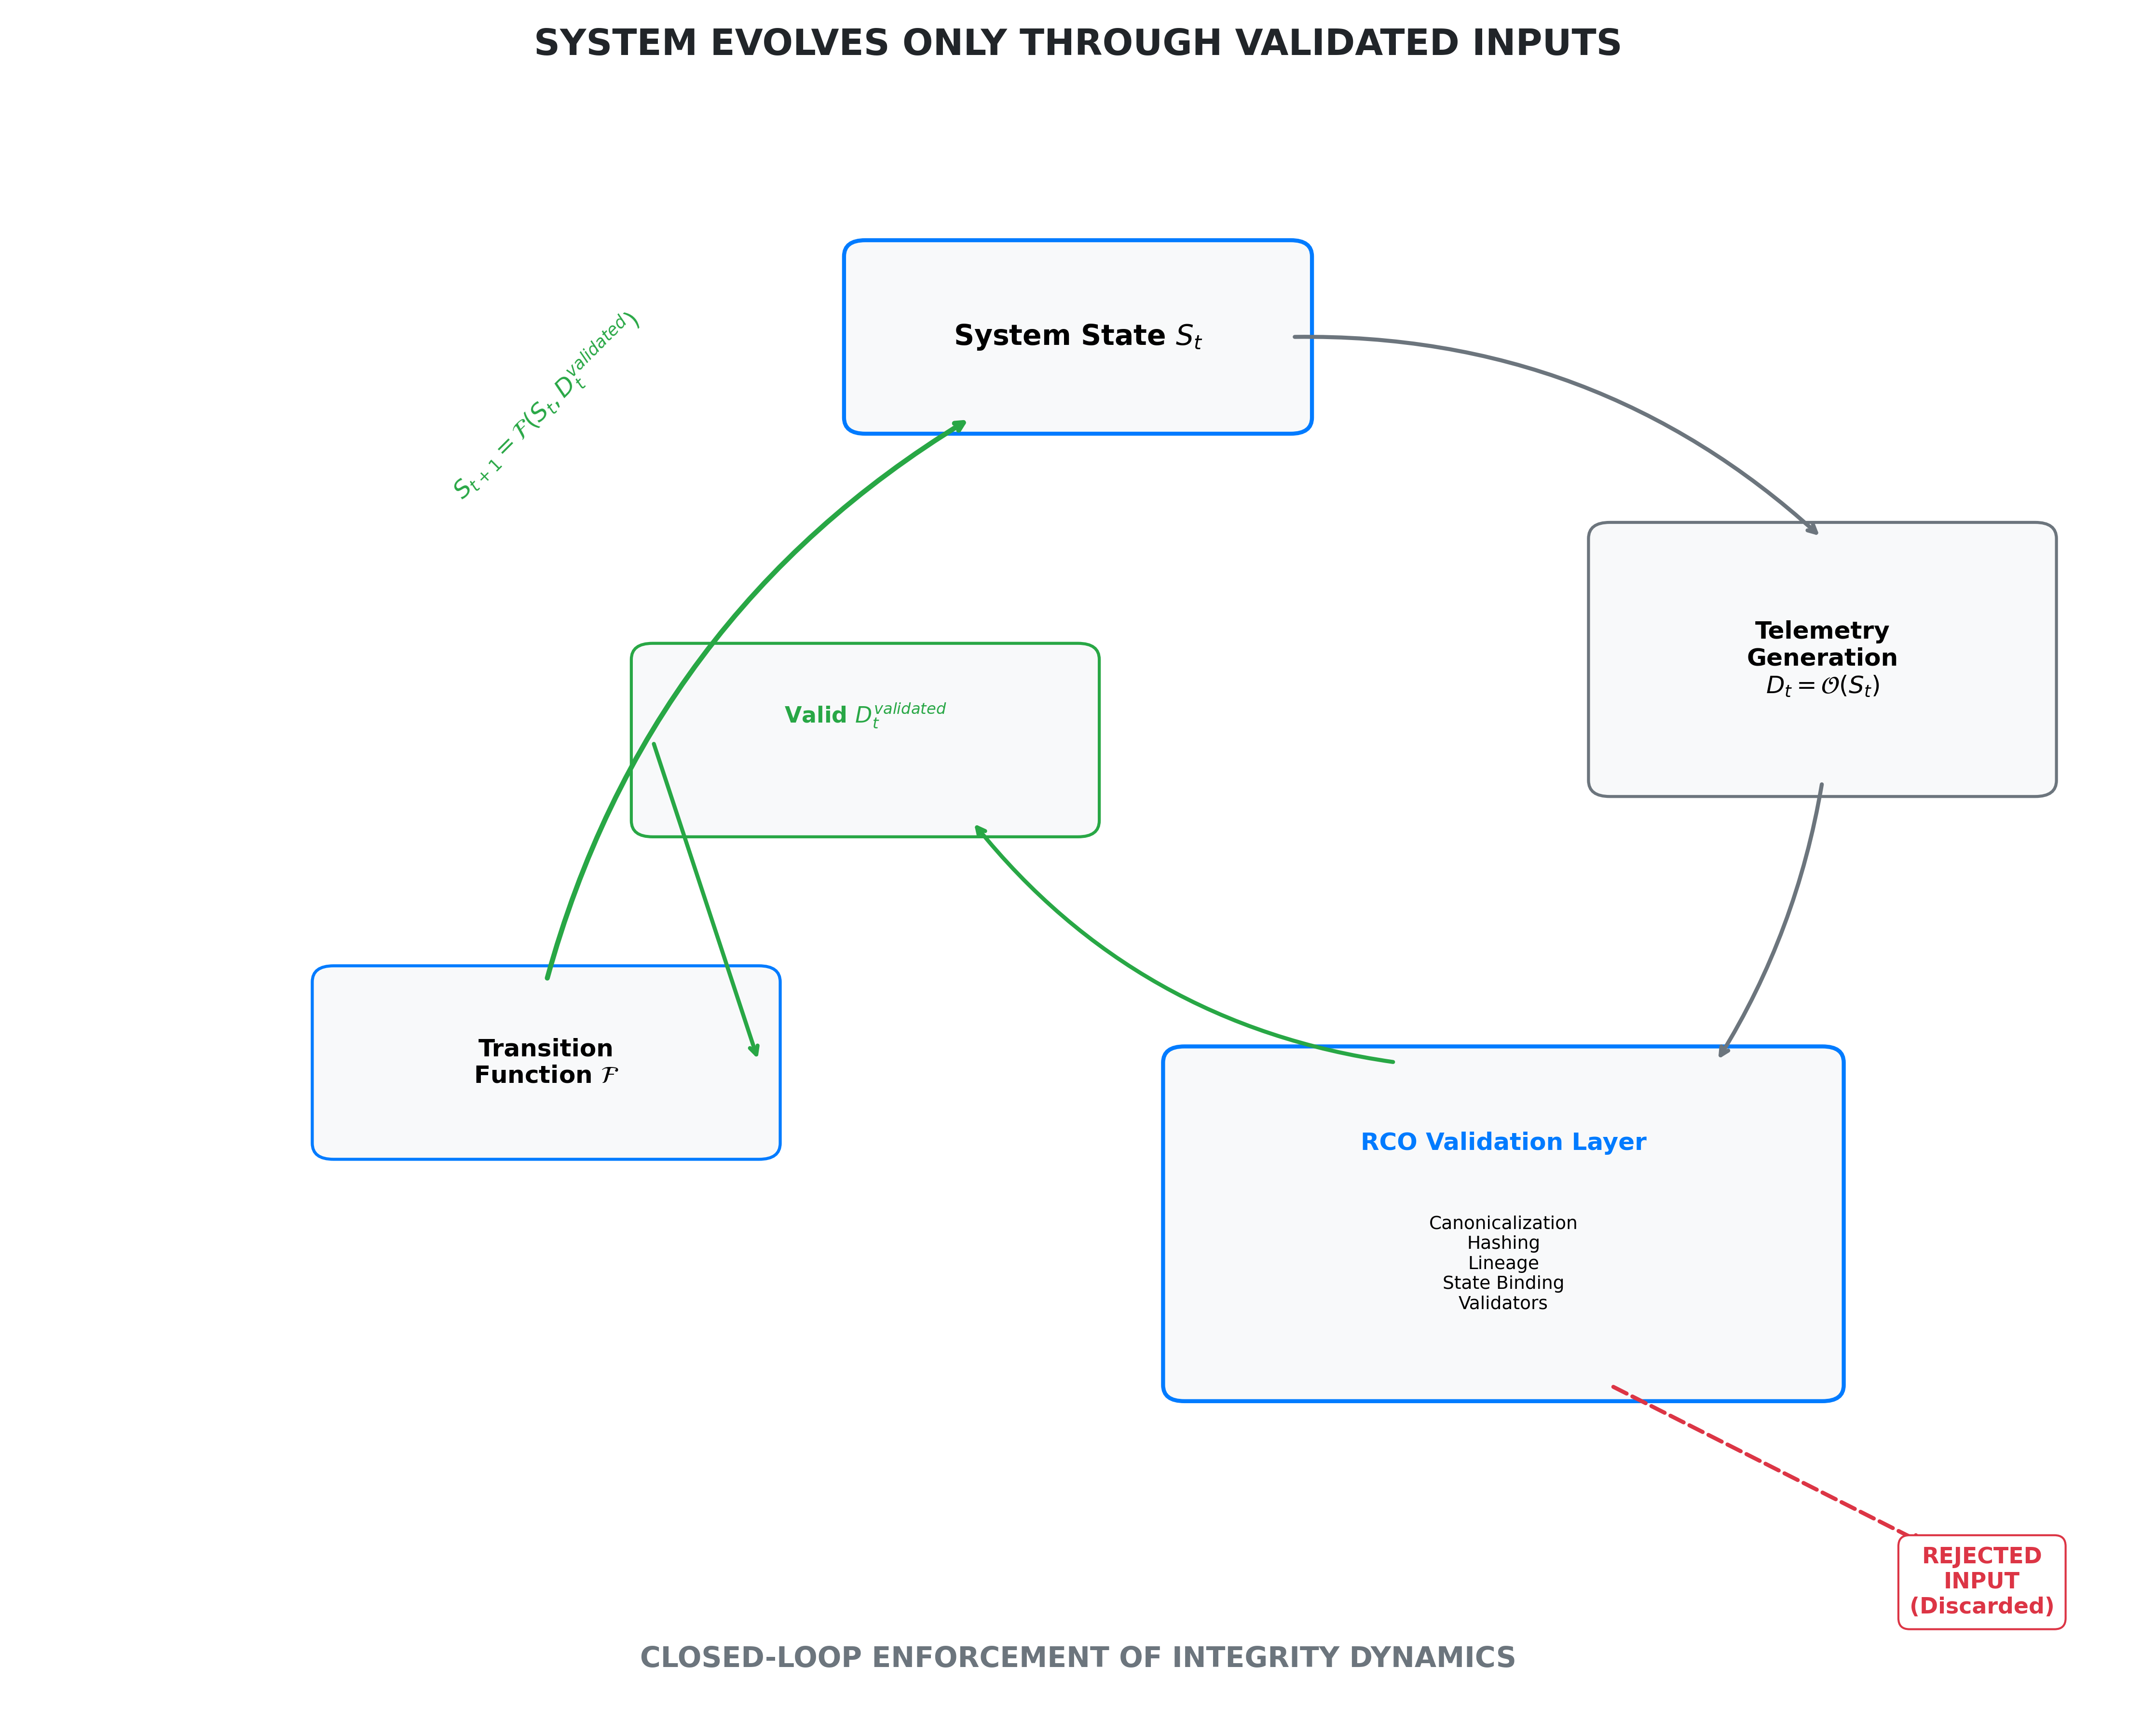
\includegraphics[width=\textwidth]{figures/2-Dimentionals/feedback_system_loop.png}
\caption{Feedback-coupled system model where state evolution is constrained by validated telemetry inputs, forming a closed-loop integrity system.}
\label{fig:feedback}
\end{figure}

Let $\mathcal{D}$ denote the space of telemetry inputs, $\mathcal{S}$ the space of system states, and $\mathcal{L}$ the lineage space. The system operates over sequences:

\begin{equation}
\{(D_t, S_t, L_t)\}_{t=0}^{T}
\end{equation}

The objective of the adversary is to produce a sequence $\{D_t'\}$ such that:

\begin{equation}
\mathcal{I}_{\text{RCO}}(D_t', L_{t-1}) = \text{accept}
\quad \text{and} \quad
D_t' \not\equiv D_t
\end{equation}

This constitutes a successful integrity violation.

\section{Adversarial Model}

We define an adversary $\mathcal{A}$ as a probabilistic polynomial-time (PPT) algorithm with access to the following capabilities:

\begin{equation}
\mathcal{A} = (\mathcal{A}_{\text{oracle}}, \mathcal{A}_{\text{network}}, \mathcal{A}_{\text{corrupt}})
\end{equation}

The oracle capability allows $\mathcal{A}$ to query the system for valid telemetry and corresponding proofs. The network capability allows interception, modification, and replay of messages. The corruption capability allows control over a subset of validator nodes.

Let $\mathcal{C} \subseteq \mathcal{V}$ denote the set of corrupted validators with $|\mathcal{C}| = f$.

\section{Security Experiment}

We define a security experiment $\text{Exp}_{\mathcal{A}}^{\text{RCO}}(\lambda)$ parameterized by a security parameter $\lambda$.

\subsection{Setup Phase}

The challenger performs the following:

\begin{enumerate}
\item Generate key shares $(K_1, \dots, K_n)$ and public key $PK$.
\item Initialize lineage state $L_0$.
\item Initialize system state $S_0$.
\end{enumerate}

\subsection{Query Phase}

The adversary may issue the following queries:

\paragraph{Telemetry Query}

\begin{equation}
\mathcal{A} \rightarrow D_t
\end{equation}

The challenger returns:

\begin{equation}
(H_t, L_t, \Sigma_t)
\end{equation}

where:

\begin{equation}
H_t = \mathcal{H}(\mathcal{S}(D_t)), \quad
L_t = \mathcal{H}(H_t \concat L_{t-1})
\end{equation}

and $\Sigma_t$ is the aggregated PoR proof.

\paragraph{Corruption Query}

The adversary may corrupt up to $f$ validators:

\begin{equation}
\mathcal{A} \rightarrow V_i
\end{equation}

and obtains $K_i$.

\paragraph{Replay Query}

The adversary may request previously generated telemetry tuples.

\subsection{Forgery Phase}

The adversary outputs $(D_t', L_{t-1}, \Sigma_t')$.

\subsection{Winning Condition}

The adversary wins if:

\begin{equation}
\text{Verify}(M_t', \Sigma_t', PK) = \text{true}
\quad \text{and} \quad
D_t' \not\equiv D_t
\end{equation}

where:

\begin{equation}
M_t' = \mathcal{H}_S(S_t') \concat L_t'
\end{equation}

\section{Security Definition}

The RCO protocol is secure if for all PPT adversaries $\mathcal{A}$:

\begin{equation}
\Pr[\text{Exp}_{\mathcal{A}}^{\text{RCO}}(\lambda) = 1] \leq \text{negl}(\lambda)
\end{equation}

\section{Attack Taxonomy}

We classify attacks into the following categories:

\subsection{Injection Attacks}

The adversary attempts to introduce arbitrary telemetry:

\begin{equation}
D_t' \in \mathcal{D}
\end{equation}

without corresponding valid state or lineage.

\subsection{Modification Attacks}

The adversary modifies valid telemetry:

\begin{equation}
D_t' = D_t + \delta_t
\end{equation}

\subsection{Replay Attacks}

The adversary reuses previously valid telemetry:

\begin{equation}
D_t' = D_k, \quad k < t
\end{equation}

\subsection{Reordering Attacks}

The adversary permutes the sequence:

\begin{equation}
D_t' = D_{\pi(t)}
\end{equation}

\subsection{State Substitution Attacks}

The adversary attempts to bind telemetry to an incorrect state:

\begin{equation}
S_t' \neq S_t
\end{equation}

\section{Security Goals}

The protocol aims to achieve the following properties:

\subsection{Integrity}

\begin{equation}
\forall D_t', \quad \text{accept}(D_t') \implies D_t' \equiv D_t
\end{equation}

\subsection{Authenticity}

\begin{equation}
\text{accept}(D_t') \implies D_t' \text{ originates from a valid system state}
\end{equation}

\subsection{Non-Repudiation}

\begin{equation}
\exists \Sigma_t \text{ such that } \text{Verify}(M_t, \Sigma_t, PK) = \text{true}
\end{equation}

\subsection{Forward Integrity}

\begin{equation}
D_k' \neq D_k \implies L_t' \neq L_t
\end{equation}

\section{Reduction Framework}

The security of the RCO protocol is reduced to the security of its underlying primitives. Let:

\begin{equation}
\epsilon_{\mathcal{H}}, \epsilon_{\mathcal{H}_S}, \epsilon_{\text{sig}}
\end{equation}

denote the probabilities of breaking the hash function, state hash, and signature scheme, respectively.

Then:

\begin{equation}
\Pr[\text{Break RCO}] \leq \epsilon_{\mathcal{H}} + \epsilon_{\mathcal{H}_S} + \epsilon_{\text{sig}} + \epsilon_{\text{threshold}}
\end{equation}

\section{Game-Based Security Interpretation}

The security experiment may be interpreted as a game between the challenger and the adversary. The adversary’s advantage is defined as:

\begin{equation}
\text{Adv}_{\mathcal{A}}^{\text{RCO}}(\lambda) =
\Pr[\text{Exp}_{\mathcal{A}}^{\text{RCO}}(\lambda) = 1]
\end{equation}

The protocol is secure if:

\begin{equation}
\text{Adv}_{\mathcal{A}}^{\text{RCO}}(\lambda) \leq \text{negl}(\lambda)
\end{equation}

\section{Implications}

This formalization establishes that any successful attack against the RCO protocol implies a break in at least one underlying cryptographic primitive or a violation of deterministic serialization. Therefore, the security of the system is tightly coupled to well-established hardness assumptions, providing strong assurance of its robustness.

\section{Conclusion}

The adversarial framework defined in this section provides a rigorous foundation for analyzing the security of the RCO protocol. By modeling the capabilities of the adversary and defining precise security goals, we establish a basis for proving that the protocol achieves strong integrity and authenticity guarantees under realistic threat models.

\section{Replay, Reordering, and Injection Resistance}

The security of the RCO protocol against replay, reordering, and injection attacks follows from the combined properties of deterministic serialization, cryptographic hashing, lineage construction, and threshold-verified Proof of Reflexion. In this section, these resistance properties are formalized through adversarial games and probability bounds, demonstrating that any successful attack implies a break in underlying cryptographic assumptions.

\subsection{Replay Attack Resistance}

A replay attack is defined as an adversarial attempt to reuse previously valid telemetry $D_k$ at a later time $t > k$ in order to induce incorrect system behavior.

\begin{figure}[htbp]
\centering
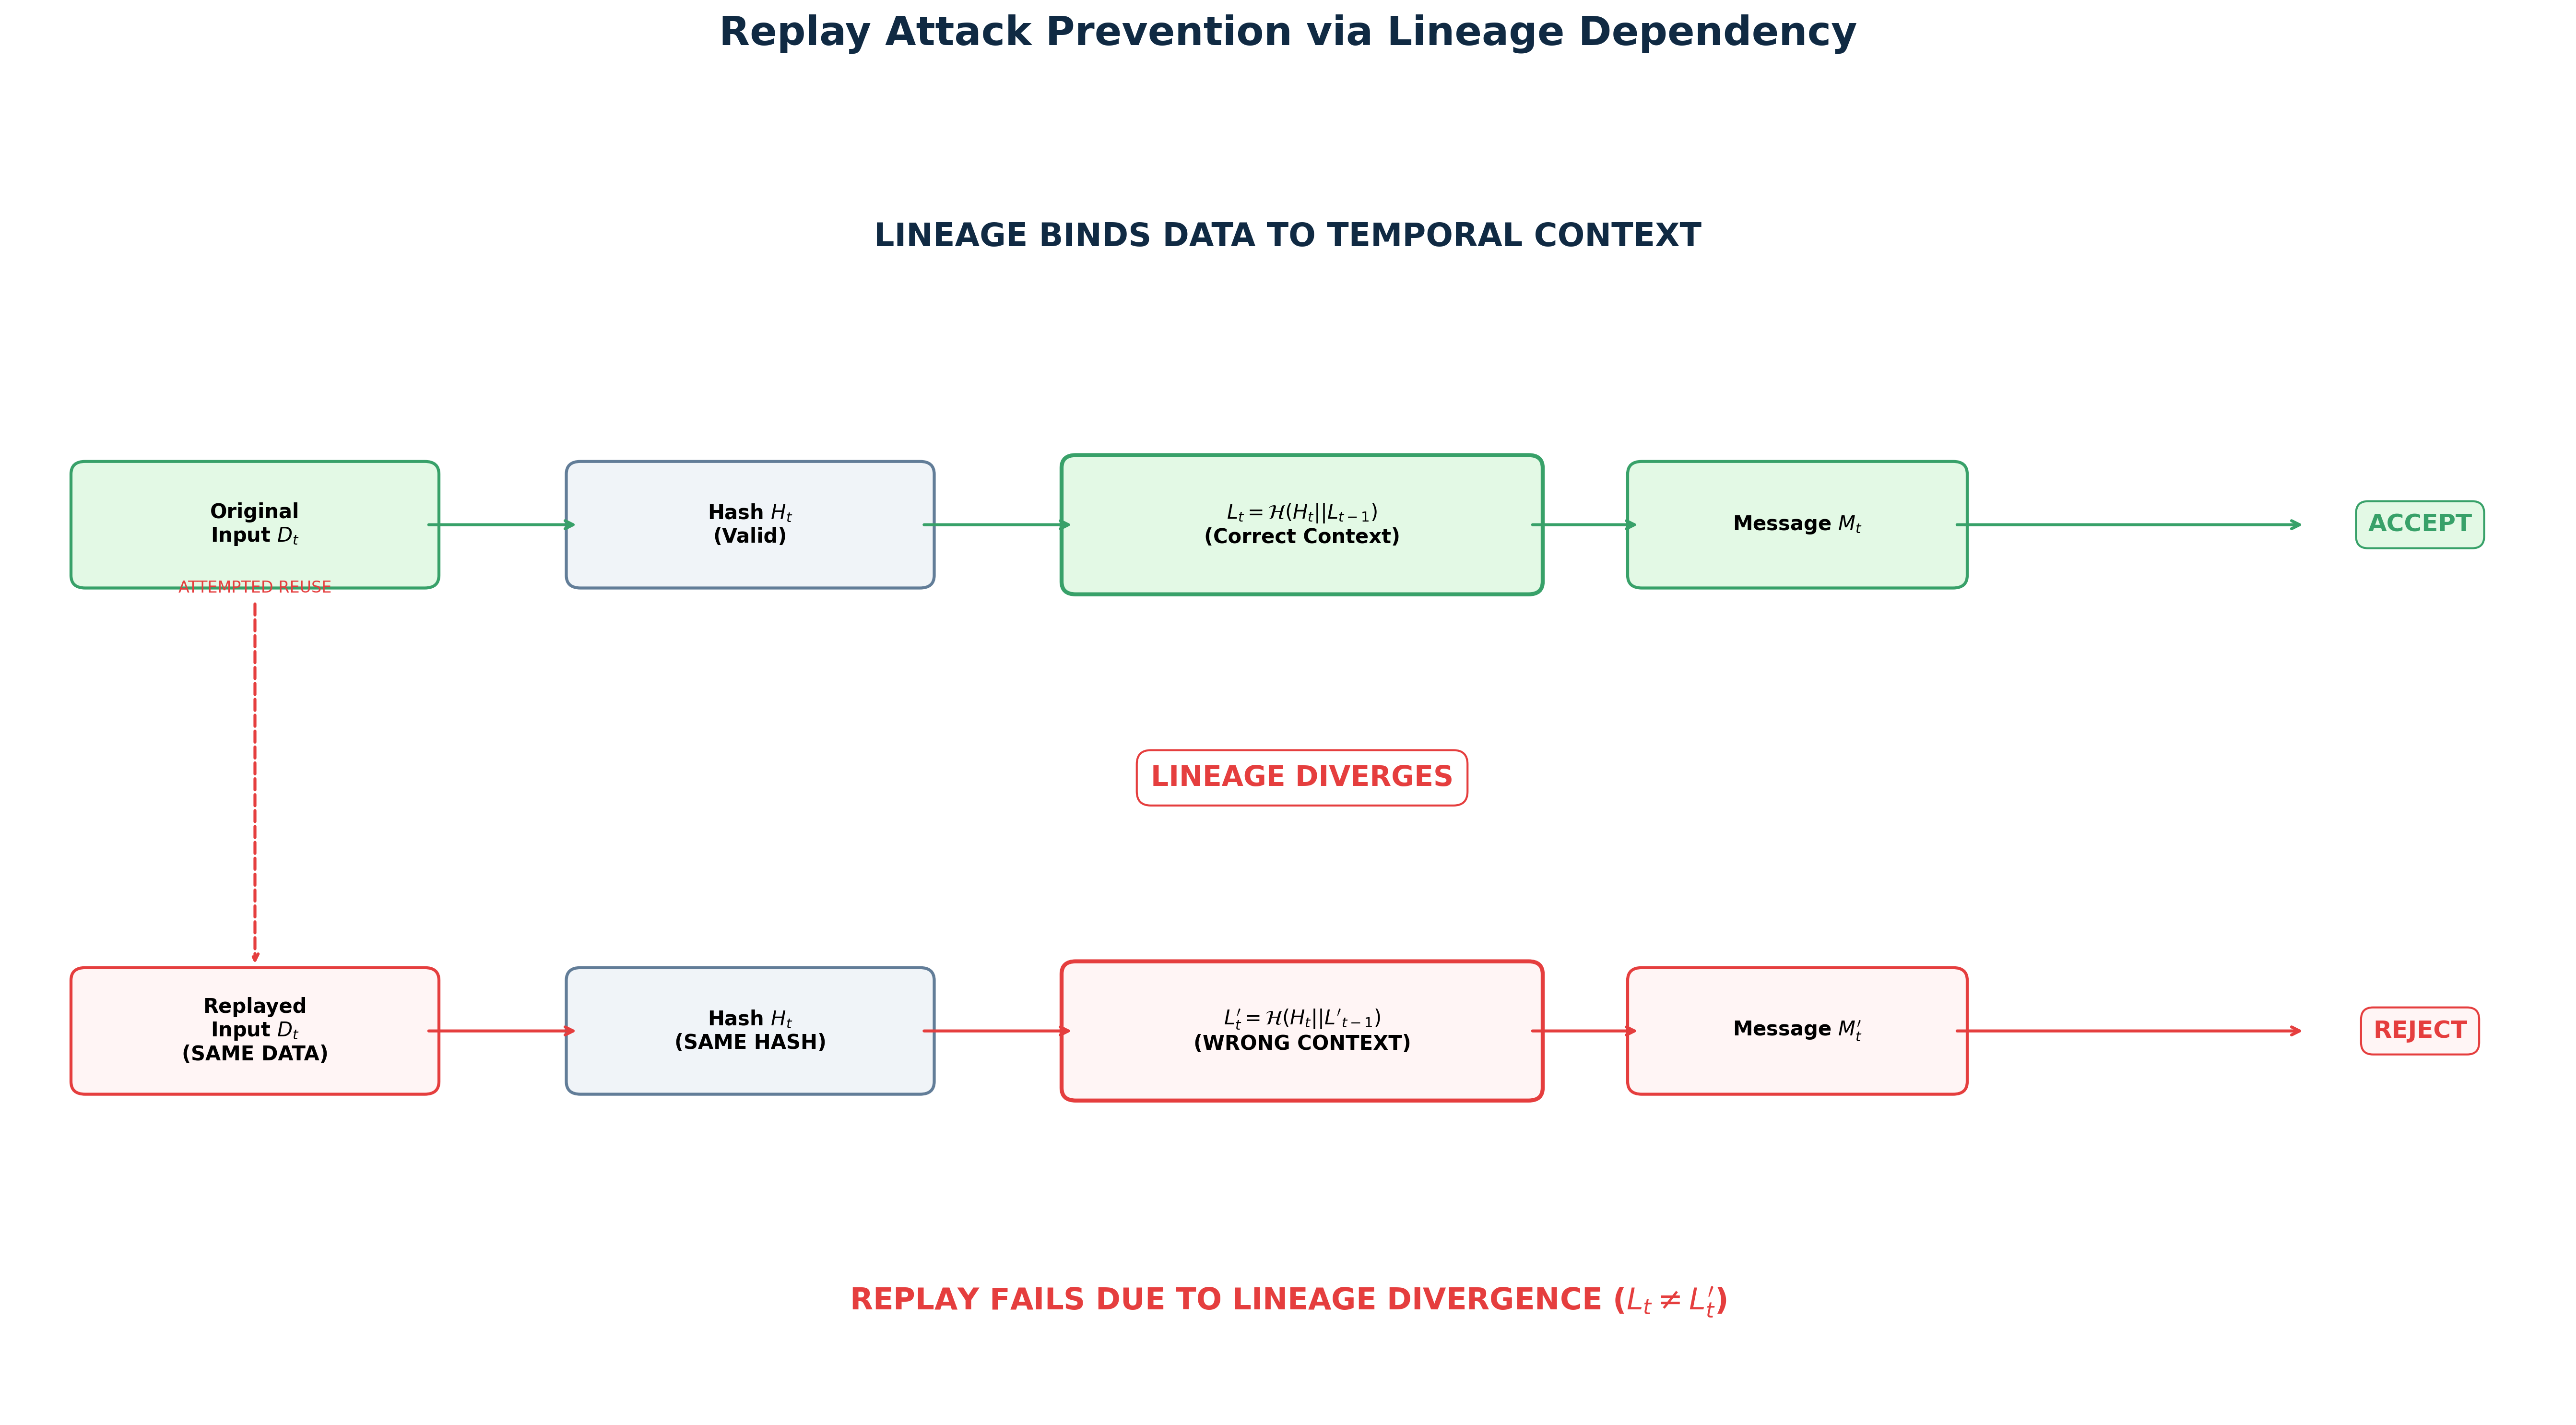
\includegraphics[width=\textwidth]{figures/2-Dimentionals/replay_prevention.png}
\caption{Replay attack prevention mechanism ensuring previously accepted telemetry cannot be reintroduced into the system.}
\label{fig:replay}
\end{figure}

\subsubsection{Replay Game Definition}

Define the replay experiment $\text{Exp}_{\mathcal{A}}^{\text{replay}}$:

\begin{enumerate}
\item The adversary obtains a valid tuple $(D_k, L_k, \Sigma_k)$.
\item The adversary constructs a replay attempt:
\begin{equation}
D_t' = D_k
\end{equation}
\item The adversary submits $(D_t', L_{t-1}, \Sigma_k)$.
\end{enumerate}

The adversary succeeds if:

\begin{equation}
\mathcal{I}_{\text{RCO}}(D_t', L_{t-1}) = \text{accept}
\end{equation}

\subsubsection{Replay Resistance Theorem}

\begin{theorem}[Replay Resistance]
Under the RCO protocol, the probability that a replayed telemetry element is accepted is negligible:
\[
\Pr[\text{Exp}_{\mathcal{A}}^{\text{replay}} = 1] \leq \epsilon_{\mathcal{H}} + \epsilon_{\text{sig}}
\]
\end{theorem}

\begin{proof}
For acceptance, the adversary must satisfy:

\begin{equation}
L_t' = \mathcal{H}(H_k \concat L_{t-1})
\end{equation}

However, the original lineage value satisfies:

\begin{equation}
L_k = \mathcal{H}(H_k \concat L_{k-1})
\end{equation}

Since $L_{t-1} \neq L_{k-1}$ for $t > k$, it follows that:

\begin{equation}
\mathcal{H}(H_k \concat L_{t-1}) \neq \mathcal{H}(H_k \concat L_{k-1})
\end{equation}

except with probability $\epsilon_{\mathcal{H}}$ due to collision resistance.

Additionally, the proof $\Sigma_k$ is bound to the message:

\begin{equation}
M_k = \mathcal{H}_S(S_k) \concat L_k
\end{equation}

For replay, the required message is:

\begin{equation}
M_t' = \mathcal{H}_S(S_t') \concat L_t'
\end{equation}

Since $L_t' \neq L_k$, $\Sigma_k$ is invalid for $M_t'$. Therefore, the adversary must forge a new signature, which succeeds with probability at most $\epsilon_{\text{sig}}$.

Thus:

\[
\Pr[\text{Replay Success}] \leq \epsilon_{\mathcal{H}} + \epsilon_{\text{sig}}
\]
\end{proof}

\subsection{Reordering Attack Resistance}

A reordering attack attempts to permute the sequence of telemetry elements to alter system behavior.

\subsubsection{Reordering Game Definition}

Let $\pi$ be a permutation over indices $\{0, \dots, t\}$. The adversary constructs:

\begin{equation}
D_t' = D_{\pi(t)}
\end{equation}

The adversary wins if:

\begin{equation}
\mathcal{I}_{\text{RCO}}(D_t', L_{t-1}) = \text{accept}
\end{equation}

\subsubsection{Reordering Resistance Theorem}

\begin{theorem}[Reordering Resistance]
Any non-trivial permutation $\pi$ results in rejection with overwhelming probability:
\[
\Pr[\text{Exp}_{\mathcal{A}}^{\text{reorder}} = 1] \leq \epsilon_{\mathcal{H}} + \epsilon_{\text{sig}}
\]
\end{theorem}

\begin{proof}
Let $H_t = \mathcal{H}(\mathcal{S}(D_t))$ and $H_t' = \mathcal{H}(\mathcal{S}(D_{\pi(t)}))$.

If $\pi(t) \neq t$, then:

\begin{equation}
H_t' \neq H_t
\end{equation}

with probability $1 - \epsilon_{\mathcal{H}}$.

The lineage requires:

\begin{equation}
L_t = \mathcal{H}(H_t \concat L_{t-1})
\end{equation}

but the adversary computes:

\begin{equation}
L_t' = \mathcal{H}(H_t' \concat L_{t-1})
\end{equation}

Thus:

\begin{equation}
L_t' \neq L_t
\end{equation}

with overwhelming probability.

Additionally, any attempt to generate a valid $\Sigma_t'$ for $L_t'$ requires forging a signature or obtaining threshold approval, which is infeasible under assumptions.

Therefore, the adversary fails except with negligible probability.
\end{proof}

\subsection{Injection Attack Resistance}

Injection attacks involve generating arbitrary telemetry $D_t'$ without corresponding legitimate state or lineage.

\subsubsection{Injection Game Definition}

The adversary outputs $(D_t', L_{t-1}, \Sigma_t')$ without querying the oracle for $D_t'$.

The adversary succeeds if:

\begin{equation}
\mathcal{I}_{\text{RCO}}(D_t', L_{t-1}) = \text{accept}
\end{equation}

\subsubsection{Injection Resistance Theorem}

\begin{theorem}[Injection Resistance]
The probability that an adversary successfully injects invalid telemetry is bounded by:
\[
\Pr[\text{Exp}_{\mathcal{A}}^{\text{inject}} = 1] \leq \epsilon_{\mathcal{H}} + \epsilon_{\mathcal{H}_S} + \epsilon_{\text{sig}} + \epsilon_{\text{threshold}}
\]
\end{theorem}

\begin{proof}
For $D_t'$ to be accepted, all of the following must hold:

\paragraph{(i) Canonical Consistency}

If $D_t' \not\equiv D_t$, then:

\begin{equation}
\mathcal{S}(D_t') \neq \mathcal{S}(D_t)
\end{equation}

implying:

\begin{equation}
\mathcal{H}(\mathcal{S}(D_t')) \neq \mathcal{H}(\mathcal{S}(D_t))
\end{equation}

except with probability $\epsilon_{\mathcal{H}}$.

\paragraph{(ii) Lineage Consistency}

The adversary must produce:

\begin{equation}
L_t' = \mathcal{H}(H_t' \concat L_{t-1})
\end{equation}

This is feasible only if $H_t'$ is correctly computed, but this does not ensure validity.

\paragraph{(iii) State Binding}

The adversary must produce a valid state $S_t'$ such that:

\begin{equation}
M_t' = \mathcal{H}_S(S_t') \concat L_t'
\end{equation}

matches the signed message. Any mismatch implies either a collision in $\mathcal{H}_S$ or inconsistency.

\paragraph{(iv) Threshold Signature}

The adversary must produce $\Sigma_t'$ such that:

\begin{equation}
\text{Verify}(M_t', \Sigma_t', PK) = \text{true}
\end{equation}

This requires either:

\begin{equation}
\text{(a)} \quad \text{Forging } t \text{ partial signatures}
\end{equation}

or:

\begin{equation}
\text{(b)} \quad \text{Compromising } t \text{ validators}
\end{equation}

Both events occur with probability at most $\epsilon_{\text{sig}}$ and $\epsilon_{\text{threshold}}$, respectively.

Combining all cases:

\[
\Pr[\text{Injection Success}] \leq \epsilon_{\mathcal{H}} + \epsilon_{\mathcal{H}_S} + \epsilon_{\text{sig}} + \epsilon_{\text{threshold}}
\]
\end{proof}

\subsection{Combined Attack Bound}

For a composite adversary attempting replay, reordering, and injection simultaneously, the success probability is bounded by:

\begin{equation}
\Pr[\text{Attack}] \leq 2\epsilon_{\mathcal{H}} + \epsilon_{\mathcal{H}_S} + 2\epsilon_{\text{sig}} + \epsilon_{\text{threshold}}
\end{equation}

which remains negligible.

\subsection{Multi-Step Adversarial Strategy Analysis}

Consider an adaptive adversary that performs a sequence of operations:

\begin{equation}
\mathcal{A} = \mathcal{A}_k \circ \dots \circ \mathcal{A}_1
\end{equation}

Each step attempts to manipulate telemetry. The success probability over $k$ steps satisfies:

\begin{equation}
\Pr[\text{Success}] \leq k \cdot (\epsilon_{\mathcal{H}} + \epsilon_{\mathcal{H}_S} + \epsilon_{\text{sig}} + \epsilon_{\text{threshold}})
\end{equation}

which remains negligible for polynomial $k$.

\subsection{Conclusion}

The RCO protocol provides strong resistance against replay, reordering, and injection attacks by combining deterministic representation, cryptographic lineage, state binding, and threshold verification. Each class of attack is reduced to breaking well-established cryptographic assumptions, ensuring that the probability of successful attack remains negligible under standard security models.

\section{State Substitution, Adaptive Adversaries, and Chosen-Message Attacks}

The integrity guarantees of the RCO protocol must hold not only against static adversaries but also against adaptive adversaries capable of interacting with the system, observing outputs, and dynamically adjusting their strategies. In particular, the Proof of Reflexion (PoR) must remain secure under chosen-message attacks and state substitution attempts, wherein the adversary attempts to bind valid lineage to an incorrect or fabricated system state.

This section formalizes these adversarial capabilities and proves that the RCO protocol remains secure under such conditions.

\subsection{State Substitution Attack Model}

A state substitution attack is defined as an attempt by the adversary to produce a valid telemetry proof for a falsified system state. Formally, the adversary attempts to construct:

\begin{equation}
(S_t', L_t, \Sigma_t')
\end{equation}

such that:

\begin{equation}
\text{Verify}(\mathcal{H}_S(S_t') \concat L_t, \Sigma_t', PK) = \text{true}
\end{equation}

while:

\begin{equation}
S_t' \neq S_t
\end{equation}

This attack targets the semantic integrity enforced by the PoR mechanism.

\subsection{PoR Security Game}

We define the PoR security experiment $\text{Exp}_{\mathcal{A}}^{\text{PoR}}$ as follows:

\begin{enumerate}
\item The challenger generates keys $(K_1, \dots, K_n)$ and public key $PK$.
\item The adversary is given access to a signing oracle:
\begin{equation}
\mathcal{O}_{\text{sign}}(S, L) \rightarrow \Sigma = \text{Aggregate}(\{\sigma_i\})
\end{equation}
\item The adversary adaptively queries the oracle with pairs $(S_i, L_i)$.
\item The adversary outputs $(S_t', L_t, \Sigma_t')$.
\end{enumerate}

The adversary wins if:

\begin{equation}
\text{Verify}(\mathcal{H}_S(S_t') \concat L_t, \Sigma_t', PK) = \text{true}
\end{equation}

and $(S_t', L_t)$ was not queried to the oracle.

\subsection{PoR Unforgeability Under Chosen-Message Attack}

\begin{theorem}[PoR EUF-CMA Security]
Assuming the underlying signature scheme is EUF-CMA secure and $\mathcal{H}_S$ is collision-resistant, the adversary’s advantage in $\text{Exp}_{\mathcal{A}}^{\text{PoR}}$ is negligible:
\[
\text{Adv}_{\mathcal{A}}^{\text{PoR}}(\lambda) \leq \epsilon_{\text{sig}} + \epsilon_{\mathcal{H}_S}
\]
\end{theorem}

\begin{proof}
Suppose $\mathcal{A}$ produces $(S_t', L_t, \Sigma_t')$ such that:

\[
\text{Verify}(\mathcal{H}_S(S_t') \concat L_t, \Sigma_t', PK) = \text{true}
\]

and $(S_t', L_t)$ was not queried.

Then $\Sigma_t'$ is a valid signature on a new message:

\[
M_t' = \mathcal{H}_S(S_t') \concat L_t
\]

This implies that $\mathcal{A}$ has either:

\begin{equation}
\text{(i)} \quad \text{forged a signature under EUF-CMA}
\end{equation}

or:

\begin{equation}
\text{(ii)} \quad \text{found } S_t \neq S_t' \text{ such that } \mathcal{H}_S(S_t) = \mathcal{H}_S(S_t')
\end{equation}

The first case occurs with probability $\epsilon_{\text{sig}}$, and the second with probability $\epsilon_{\mathcal{H}_S}$.

Thus:

\[
\text{Adv}_{\mathcal{A}}^{\text{PoR}} \leq \epsilon_{\text{sig}} + \epsilon_{\mathcal{H}_S}
\]
\end{proof}

\subsection{Adaptive Adversary Model}

An adaptive adversary $\mathcal{A}$ can:

\begin{enumerate}
\item Observe prior telemetry $(D_1, \dots, D_{t-1})$,
\item Query signing oracles on chosen states,
\item Corrupt validators dynamically,
\item Select attack targets based on observed outputs.
\end{enumerate}

Formally, the adversary operates as:

\begin{equation}
\mathcal{A} = (\mathcal{A}_1 \rightarrow \mathcal{A}_2 \rightarrow \dots \rightarrow \mathcal{A}_k)
\end{equation}

where each stage depends on previous outputs.

\subsection{Adaptive Corruption Model}

Let $\mathcal{C}_t$ denote the set of corrupted validators at time $t$. The adversary may expand $\mathcal{C}_t$ over time:

\begin{equation}
\mathcal{C}_1 \subseteq \mathcal{C}_2 \subseteq \dots \subseteq \mathcal{C}_t
\end{equation}

subject to:

\begin{equation}
|\mathcal{C}_t| < t
\end{equation}

to remain below the threshold.

\subsection{Security Under Adaptive Corruption}

\begin{theorem}[Adaptive Threshold Security]
If at all times $|\mathcal{C}_t| < t$, then the adversary cannot produce a valid aggregated signature for any new message.
\end{theorem}

\begin{proof}
At time $t$, the adversary controls $f < t$ validators. To produce a valid aggregated signature, the adversary must obtain at least $t$ valid partial signatures.

Since honest validators sign only valid messages, the adversary must either:

\begin{equation}
\text{(i)} \quad \text{convince honest validators to sign invalid messages}
\end{equation}

or:

\begin{equation}
\text{(ii)} \quad \text{forge signatures for missing shares}
\end{equation}

The first case is prevented by deterministic validation rules. The second contradicts EUF-CMA security.

Thus, the adversary fails.
\end{proof}

\subsection{Chosen-Message Attack on Lineage}

An adversary may attempt to construct a lineage collision under chosen inputs. Let the adversary select $D_t'$ such that:

\begin{equation}
\mathcal{H}(\mathcal{S}(D_t')) = \mathcal{H}(\mathcal{S}(D_t))
\end{equation}

This is equivalent to finding a collision in $\mathcal{H}$, which succeeds with probability $\epsilon_{\mathcal{H}}$.

\subsection{Hybrid Argument for Full Security}

We now construct a hybrid argument to prove full system security.

\paragraph{Hybrid 0: Real System}

The adversary interacts with the full RCO system.

\paragraph{Hybrid 1: Replace $\mathcal{H}$ with Random Oracle}

The adversary’s advantage changes by at most $\epsilon_{\mathcal{H}}$.

\paragraph{Hybrid 2: Replace $\mathcal{H}_S$ with Random Oracle}

Advantage changes by at most $\epsilon_{\mathcal{H}_S}$.

\paragraph{Hybrid 3: Replace Signature Scheme with Ideal Function}

Advantage changes by at most $\epsilon_{\text{sig}}$.

\paragraph{Conclusion}

In the ideal system, the adversary has no advantage. Therefore:

\begin{equation}
\text{Adv}_{\mathcal{A}}^{\text{RCO}} \leq \epsilon_{\mathcal{H}} + \epsilon_{\mathcal{H}_S} + \epsilon_{\text{sig}} + \epsilon_{\text{threshold}}
\end{equation}

\subsection{Multi-Round Adaptive Attack Bound}

For an adversary performing $q$ adaptive queries:

\begin{equation}
\text{Adv}_{\mathcal{A}}^{(q)} \leq q \cdot (\epsilon_{\mathcal{H}} + \epsilon_{\mathcal{H}_S} + \epsilon_{\text{sig}} + \epsilon_{\text{threshold}})
\end{equation}

which remains negligible for polynomial $q$.

\subsection{State Consistency Guarantee}

The PoR mechanism ensures:

\begin{equation}
\text{accept}(D_t') \implies \exists S_t \text{ such that } D_t' = \mathcal{G}(S_t)
\end{equation}

Thus, state substitution is prevented.

\subsection{Conclusion}

The RCO protocol remains secure under strong adversarial models including adaptive corruption, chosen-message attacks, and state substitution attempts. The Proof of Reflexion, combined with threshold cryptography and deterministic lineage construction, ensures that any successful attack implies a break in underlying cryptographic primitives, thereby providing strong assurance of system integrity.

\section{System-Level Security: Composability, Liveness, and Failure Modes}

The RCO protocol operates as a composition of multiple cryptographic and distributed components, each of which enforces a specific integrity invariant. While previous sections establish the security of individual components, system-level security requires that these guarantees are preserved under composition, concurrent execution, and partial system failures. This section formalizes the composability of the protocol, analyzes the trade-offs between safety and liveness, and defines the boundaries under which the system maintains its security guarantees.

\subsection{Composability Model}

Let $\mathcal{P}_{\text{core}}$ denote the cryptographic core pipeline and $\mathcal{I}_{\text{RCO}}$ the ingestion pipeline. The full system is defined as:

\begin{equation}
\mathcal{P}_{\text{system}} = \mathcal{P}_{\text{core}} \circ \mathcal{I}_{\text{RCO}}
\end{equation}

Each component enforces a local invariant:

\begin{equation}
\mathcal{P}_{\text{core}}: \text{Valid}_{\text{core}}(D_t)
\end{equation}

\begin{equation}
\mathcal{I}_{\text{RCO}}: \text{Valid}_{\text{ingest}}(D_t)
\end{equation}

The composed system enforces:

\begin{equation}
\text{Valid}_{\text{system}}(D_t) = \text{Valid}_{\text{core}}(D_t) \land \text{Valid}_{\text{ingest}}(D_t)
\end{equation}

\subsection{Universal Composability Property}

\begin{theorem}[Composability of RCO]
If each component of the RCO protocol satisfies its respective security definition under standard cryptographic assumptions, then the composed system $\mathcal{P}_{\text{system}}$ is secure.
\end{theorem}

\begin{proof}
Assume an adversary $\mathcal{A}$ breaks $\mathcal{P}_{\text{system}}$. Then $\mathcal{A}$ must violate either:

\begin{equation}
\text{Valid}_{\text{core}}(D_t) \quad \text{or} \quad \text{Valid}_{\text{ingest}}(D_t)
\end{equation}

If $\text{Valid}_{\text{core}}(D_t)$ is violated, then $\mathcal{A}$ breaks one of the cryptographic primitives: $\mathcal{S}$, $\mathcal{H}$, $\mathcal{H}_S$, or the signature scheme.

If $\text{Valid}_{\text{ingest}}(D_t)$ is violated, then $\mathcal{A}$ breaks threshold security or deterministic verification.

Thus, any successful attack reduces to breaking a component, which occurs with negligible probability. Therefore, the composed system is secure.
\end{proof}

\subsection{Sequential Composition Under Concurrency}

Let multiple ingestion pipelines operate concurrently:

\begin{equation}
\mathcal{I}_1, \mathcal{I}_2, \dots, \mathcal{I}_m
\end{equation}

Each produces candidate telemetry sequences. The global system enforces a deterministic merge:

\begin{equation}
D_t = \min_{\prec} \{D_t^{(1)}, \dots, D_t^{(m)}\}
\end{equation}

Since $\prec$ is derived from canonical serialization, all nodes agree on the selected element. Therefore, concurrency does not introduce divergence.

\subsection{Safety and Liveness Definitions}

We define two fundamental system properties:

\paragraph{Safety}

\begin{equation}
\text{No invalid telemetry is ever accepted}
\end{equation}

Formally:

\begin{equation}
\forall t, \quad \mathcal{I}_{\text{RCO}}(D_t, L_{t-1}) = \text{accept} \implies D_t \text{ is valid}
\end{equation}

\paragraph{Liveness}

\begin{equation}
\text{All valid telemetry is eventually accepted}
\end{equation}

Formally:

\begin{equation}
\forall D_t \text{ valid}, \quad \exists t' \geq t \text{ such that } \mathcal{I}_{\text{RCO}}(D_t, L_{t'-1}) = \text{accept}
\end{equation}

\subsection{Safety-Liveness Tradeoff}

The RCO protocol prioritizes safety over liveness. In particular:

\begin{equation}
\text{If verification is inconclusive, then } \mathcal{I}_{\text{RCO}} = \text{reject}
\end{equation}

This ensures that:

\begin{equation}
\text{Safety is absolute} \quad \text{and} \quad \text{Liveness is conditional}
\end{equation}

\subsection{Liveness Under Honest Majority}

\begin{theorem}[Liveness Guarantee]
If at least $t$ validators are honest and the network is eventually synchronous, then all valid telemetry is eventually accepted.
\end{theorem}

\begin{proof}
Honest validators produce valid partial signatures for valid telemetry. Once $t$ such signatures are available, aggregation yields a valid $\Sigma_t$. Eventual synchrony ensures that these signatures are propagated to all nodes. Therefore, $\mathcal{I}_{\text{RCO}}$ returns accept.
\end{proof}

\subsection{Failure Modes}

We now characterize the conditions under which the system may fail.

\subsubsection{Threshold Failure}

If:

\begin{equation}
|\mathcal{C}| \geq t
\end{equation}

then adversaries can produce valid signatures for arbitrary messages, violating integrity.

\subsubsection{Cryptographic Break}

If any primitive is broken:

\begin{equation}
\epsilon_{\mathcal{H}} \approx 1 \quad \text{or} \quad \epsilon_{\text{sig}} \approx 1
\end{equation}

then security collapses.

\subsubsection{Serialization Failure}

If $\mathcal{S}$ is not canonical:

\begin{equation}
D_1 \equiv D_2 \not\implies \mathcal{S}(D_1) = \mathcal{S}(D_2)
\end{equation}

then deterministic guarantees fail.

\subsubsection{Network Partition}

In a partitioned network, different subsets of validators may produce conflicting partial signatures. However, without reaching threshold $t$, no conflicting telemetry is accepted, preserving safety at the cost of liveness.

\subsection{Byzantine Resilience Boundary}

The system tolerates up to:

\begin{equation}
f < t
\end{equation}

Byzantine validators. Beyond this threshold, the adversary can control acceptance.

\subsection{Graceful Degradation}

Under partial failure, the system degrades gracefully:

\begin{equation}
\text{Failure} \implies \text{reduced liveness, not reduced safety}
\end{equation}

\subsection{End-to-End System Guarantee}

\begin{theorem}[System Integrity]
Under the assumptions:
\begin{enumerate}
\item $f < t$,
\item $\mathcal{H}, \mathcal{H}_S$ are collision-resistant,
\item the signature scheme is EUF-CMA secure,
\item $\mathcal{S}$ is canonical,
\end{enumerate}
the RCO system satisfies:

\[
\forall t, \quad \text{accept}(D_t) \implies D_t \text{ is valid}
\]
\end{theorem}

\begin{proof}
Follows from composability of core and ingestion guarantees, and threshold security.
\end{proof}

\subsection{Compositional Stability}

Let the system operate over $T$ steps. The cumulative failure probability satisfies:

\begin{equation}
\Pr[\text{Failure over } T] \leq T \cdot (\epsilon_{\mathcal{H}} + \epsilon_{\mathcal{H}_S} + \epsilon_{\text{sig}} + \epsilon_{\text{threshold}})
\end{equation}

which remains negligible for polynomial $T$.

\subsection{Conclusion}

The RCO protocol achieves strong system-level security through the composition of deterministic serialization, cryptographic lineage, Proof of Reflexion, and threshold verification. The protocol guarantees safety under all conditions and liveness under standard network assumptions, while clearly defining the boundaries under which these guarantees hold. This establishes the protocol as a robust and formally verified framework for secure telemetry ingestion in adversarial environments.